\chapter{Modeling}
\label{ch:modeling}

In this section, we aim to discuss our choice of model architectures and how we utilized them in our solution. Beyond direct data manipulation, we also addressed the issue of severe class imbalance using advanced techniques designed to accommodate such imbalance and guide the model toward strong performance in detecting malignant lesions. We thoroughly examine the models, loss functions, class weighting strategies, model training, and the linear probing of selected models, as well as how we incorporated segmentation-aided training to support the fine-tuning process. Last section will discuss model fairness and how we design domain-aware training given the skin color groups/types.

\section{Model architectures}
\subsection{ConvNeXt}
ConvNeXt \cite{convnext2022} model architecture is a convolutional neural network architecture combining ideas of standard ConvNets with design principles inspired by transformer-based models like Vision Transformers (ViTs). It retains the efficiency and inductive biases of CNNs (like translation equivariance) while incorporating modern improvements such as large kernel sizes, layer normalization, and inverted bottlenecks. 
ConvNeXt models were supervisedly pretrained on the large-scale ImageNet-21K dataset and some were fine-tuned on ImageNet-1k. Best model achieved 87.8 acc@1 on ImageNet1k.

We thought of it as a good starting point due to several reasons: inductive biases, transfer learning, good performance on moderately sized datasets, and availability of papers using it for medical image processing( \cite{MedNeXt}, \cite{liu2023deep}).

\subsection{ConvNeXtV2}
The obvious next model to try was the ConvNeXtV2 architecture \cite{convnext_v2_2023}, a direct improvement over the original ConvNeXt. It leverages unsupervised pretraining via masked image modeling technique inspired by masked autoencoders in which the training objective is for the model to reconstruct the occluded parts of an image. Through this reconstruction-based pretraining, the model learns more effective feature representations. This was validated by experiments in which ConvNeXtV2 outperformed its predecessor on ImageNet-1K, achieving a then state-of-the-art accuracy of 88.9\%

What particularly drew our attention was the availability of fine-tuning recipes for a variety of tasks. These pretrained models performed well on downstream tasks such as classification, segmentation, and object detection, making ConvNeXtV2 a logical next choice for our problem.

\subsection{EfficientNetV2}

EfficientNetV2 \cite{efficientnetv2} is a family of CNN's that builds on the original EfficientNet architecture by introducing faster training, improved accuracy, and better scalability. It combines compound model scaling with progressive learning strategies and uses Fused-MBConv blocks in early layers for speed, while maintaining MBConv blocks in deeper layers for representational power. 
The model achieved 88.5\% accuracy on the ImageNet-1K dataset.

Our decision to explore EfficientNetV2 as one of the core architectures in our experiments was strongly motivated by its extensive adoption in the ISIC 2020 Challenge submissions. A large portion of the top-ranked solutions in that competition utilized one or more variants of EfficientNet, often as part of an ensemble, demonstrating the architecture’s practical effectiveness in skin lesion classification tasks. This widespread usage and good performance on this domain made it a logic choice to explore.


\subsection{DinoV2}

DINOv2 \cite{dinov2} is a self-supervised vision transformer model trained using the DINO (Self-Distillation with No Labels) framework. DINOv2 learns visual representations without labeled data by using a teacher-student training setup in which both networks process multiple views of the same image. The student network is trained to match the output of the teacher network, which is updated via exponential moving averages. This method encourages the model to learn semantically rich features.

DINOv2 is considered a foundation model in computer vision. As it was pretrained on a large-scale unlabeled dataset, the features obtained from the frozen DINOv2 can be used for linear probing, which means a classification head is attached to a model utilizing DINOv2 as the backbone and trained on top of its features to perform a downstream classification task. The idea is that DINOv2 features are semantically rich enough for the classification head to perform well.

It is also worth knowing that the authors in the ablation studies concluded that the model showcased no clear patterns indicating bias towards gender, skintones or age.

In the following figure from the original article, we can see how the first few PCA components of those features look like:

\begin{figure}[htbp]
\centering
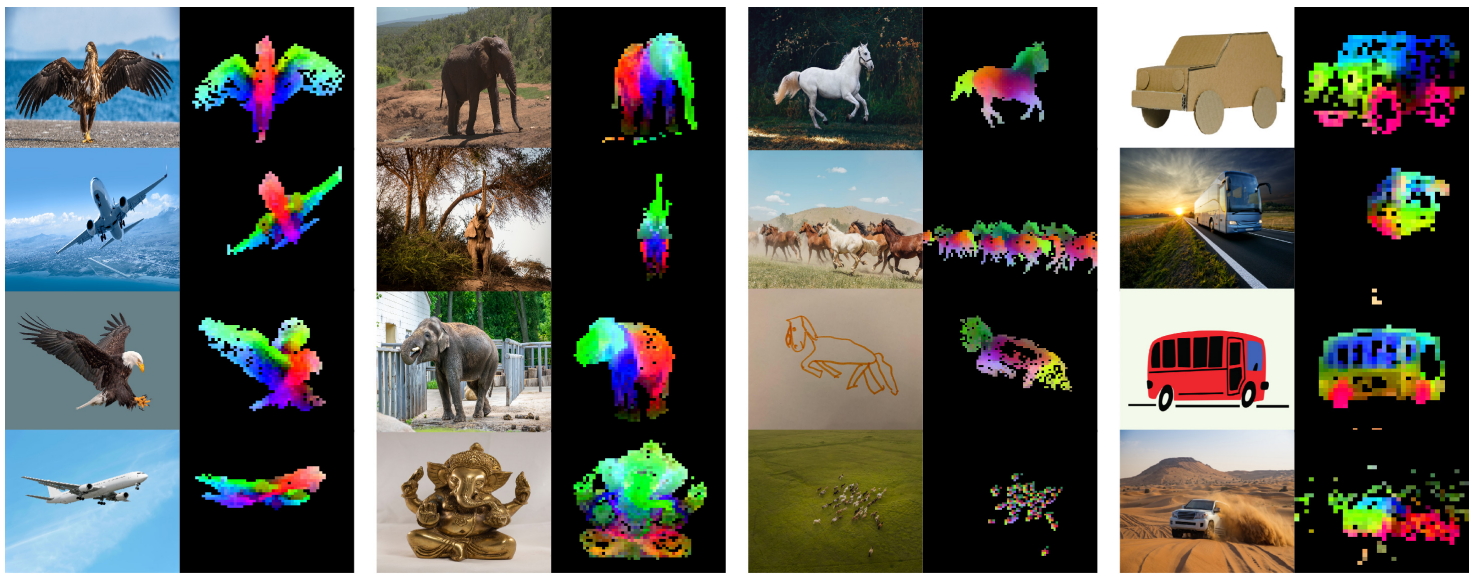
\includegraphics[width=0.9\linewidth]{figures/dino_pca_comp_of_features.png}
\caption{Visualization of the first few PCA components of DINOv2 features (from the original DINOv2 paper)}
\label{fig:dino-pca}
\end{figure}


In our setting, we utilize DINOv2 in a linear probing setup. The backbone was frozen, and we trained only a lightweight classifier head on top of the extracted features. Since the majority of our models were prone to overfitting due to severe class imbalance, we believed this frozen-backbone setup could be particularly beneficial for achieving better generalization performance on our dataset.

\section{Loss functions and class weighting}

The ISIC 2020 challenge dataset has a 49-to-1 ratio of benign to malignant images. We tackled this issue using several dataset-level techniques (namely, oversampling, transformations of malignant images, etc.) as well as training-level sampling strategies (such as balanced batch samplers and oversamplers).

A common approach in computer vision tasks is to address this imbalance through custom loss functions that guide the model to focus either on harder-to-classify examples, on minority class samples, or on improving recall. In this section, we discuss how we used custom training objectives to increase the recall and F1 score for malignant class predictions.

\subsection{Cross-entropy}
As shown by \cite{dynamic_loss_balancing}, authors suggest that the interpretation of the standard cross-entropy loss is that it is a negative logarithm of the geometric mean of the correct class posterior:
\begin{myequation}
\caption{Cross-entropy as the negative log of the geometric mean of posteriors}
\label{eq:ce_geom}
\[
\text{CE} = -\frac{1}{N} \sum_{n=1}^{N} \ln P_n^{y_n} 
= -\frac{1}{N} \ln \prod_{n=1}^{N} P_n^{y_n} 
= -\ln \left( \prod_{n=1}^{N} P_n^{y_n} \right)^{\frac{1}{N}} 
= -\ln \overline{P}
\]
\end{myequation}


Cross entropy can also be view as summation of geometric means $P_c$ over all classes:
\begin{myequation}
\caption{Cross-entropy as a sum over class-wise log posteriors}
\label{eq:ce_weighted}
\[
\text{CE} = -\frac{1}{N} \sum_{c=1}^{C} \sum_{n: y_n = c} \ln P_n^c 
= -\sum_{c=1}^{C} \frac{1}{N} \ln \prod_{n: y_n = c} P_n^c 
= -\sum_{c=1}^{C} \frac{N_c}{N} \ln \left( \prod_{n: y_n = c} P_n^c \right)^{\frac{1}{N_c}} 
= -\sum_{c=1}^{C} \frac{N_c}{N} \ln \overline{P_c}
\]
\end{myequation}

Here, the set $\{n : y_n = c\}$ denotes all training examples belonging to class $c$, and $P_c = \left( \prod_{n: y_n = c} P_n^{y_n} \right)^{1/N_c}$ is the geometric mean of the predicted posteriors for class $c$.

As shown by equation~\eqref{eq:ce_weighted}, standard cross-entropy maximizes the arithmetic mean of the posterior geometric mean per class, with weights of each mean being occurrences of that class in the dataset. For any class imbalanced task, such partitioning is harmful as the bias for the majority class could prevail, which would result in the model always, or too often, predicting majority class/classes.


\subsection{Inverse Frequency Weighting (IFW)}

There are a couple of remedies for the imbalance problem shown in Equation~\eqref{eq:ce_weighted}.

Since cross-entropy can be expressed as
\begin{myequation}
\caption{Weighted cross-entropy expressed with per-class geometric means}
\label{eq:ce_weighted_2}
\[
\text{CE} = -\sum_{c=1}^{C} \frac{N_c}{N} \ln \overline{P_c}
\]
\end{myequation}
the first solution that comes to mind is to cancel out the weighting coefficients $\frac{N_c}{N}$. The technique known as inverse frequency weighting is a method of adjusting class contributions, where we multiply the biased weights in Equation~\eqref{eq:ce_weighted_2} by $\frac{N}{N_c} \cdot \alpha$, that is, by the inverse class frequency scaled by a factor $\alpha$, referred to as the correction coefficient, which is a training hyperparameter.

When using IFW cross entropy, equation~\eqref{eq:ce_weighted_2} deteriorates to : 
\begin{myequation}
\caption{IFW cross-entropy formula}
\label{eq:ce_ifw}
\[
\text{CE}_{\text{IFW}} = -\sum_{c=1}^{C} w_c \cdot \frac{N_c}{N} \ln P_c 
= -\sum_{c=1}^{C} \alpha \ln P
\]
\end{myequation}


\subsection{Recall-Based Cross-Entropy Loss}

As pointed out in \cite{dynamic_loss_balancing}, increasing the weights of minority classes can lead to a significant rise in false positives. The reason behind this is that standard cross-entropy is designed to consider only the posterior probability of the true class while ignoring the distribution over incorrect classes. This makes it suboptimal for our task, where we face a severe positive-to-negative class imbalance. For example, assigning 50 times more weight to malignant examples than benign ones can theoretically, and has experimentally, proven problematic, as it results in a surge of false positives. This often yields a recall of 1.00 but with extremely low precision.

To address this, \cite{dynamic_loss_balancing} proposes adapting loss weights based on the model’s recall performance. The idea is to begin training with inverse frequency-weighted cross-entropy and gradually reduce the weight assigned to the malignant class as its recall approaches 1.00. This allows the model to continue learning even after achieving perfect recall, ensuring gradient flow through the network, particularly to improve precision. In our case, the priority is to maximize recall for malignant examples, accepting the risk of lower precision, since class-imbalance techniques are intended to mitigate such trade-offs.
The exact equation follows:

\begin{myequation}
\caption{Recall-based class weighting formula}
\label{eq:recall_weight}
\[
w^{R}_{c,t} = \frac{N}{N_c} \left( 1 - R_{c,t} \right) + \epsilon
\]
\end{myequation}


Let us consider a simple example. Suppose we have a 50-to-1 negative-to-positive class ratio in a dataset with 10 malignant (positive) and 50 benign (negative) samples. If the model achieves a recall of 1.00 but produces 30 false positives, the resulting precision would be:
\[
\text{Precision} = \frac{10}{10 + 30} = 0.25 \quad (25\%)
\]
and the F1-score would be:
\[
\text{F1-score} = 2 \cdot \frac{\text{Precision} \cdot \text{Recall}}{\text{Precision} + \text{Recall}} = 2 \cdot \frac{0.25 \cdot 1.00}{0.25 + 1.00} = 0.40 \quad (40\%)
\]
However, one could argue that a 10\% false positive rate may be acceptable in our setting, given the importance of correctly identifying malignant cases.


\subsection{Online Hard Example Mining (OHEM)}

OHEM \cite{ohem} is a loss function technique originally designed for training deep neural networks on object detection tasks. It is based on the principle of distinguishing between easy-to-classify and hard-to-classify examples, with the goal of selecting and prioritizing the latter during training.

The objective of OHEM is to optimize model performance by focusing training on harder examples, rather than treating all examples equally. 

The training procedure involves calculating per-sample loss within each mini-batch, identifying the hardest examples (i.e., those with the highest loss values), and emphasizing them in subsequent training steps. These hard examples contribute more significantly to the gradient updates, as their higher loss values result in larger gradients, pushing the model to focus more on learning from them.

\subsection{Focal Loss}

Focal loss, proposed by \cite{focal_loss}, is a modified version of the standard cross-entropy loss designed to down-weight the contribution of well-classified examples and focus learning on hard, misclassified ones.

The authors argue that easily classified examples dominate the loss and gradients during training, which can stop learning, especially when a large class imbalance is present. While inverse-frequency weighting can address class imbalance, and methods like OHEM can be combined with it to focus on hard examples, such strategies may still lead to a bias toward misclassifying positive examples without explicitly addressing the rise in false positives. Focal loss addresses this by dynamically scaling the loss and reducing the contribution of easy negatives, thus acting as a balancing mechanism that emphasizes hard negatives during training.

The focal loss is defined as:
\begin{myequation}[H]
\caption{The focal loss formula}
\label{eq:focal_loss}
\[
\text{FL}(p_t) = - \alpha (1 - p_t)^{\gamma} \log(p_t)
\]
\end{myequation}

where:
\begin{itemize}
  \item \( p_t \) is the model’s estimated probability for the true class.
  \item \( \alpha \in [0, 1] \) is a balancing factor that compensates for class imbalance.
  \item \( \gamma \geq 0 \) is the focusing parameter that controls the rate at which easy examples are down-weighted.
\end{itemize}

The term \( (1 - p_t)^{\gamma} \) is the modulating factor that reduces the loss contribution of well-classified examples (i.e., those with high \( p_t \)).

Additionally, the authors experimented with introducing class priors into the model itself, ensuring that the estimated probability \( p \) for rare classes remains low at initialization. This helps shift early learning focus toward underrepresented (minority) classes.


\section{Probing vs fine-tuning}

In the model subsections, we stated that DINOv2 is a foundation model with large-scale pretraining that yields semantically rich image features suitable for linear probing. We implemented logic to freeze the model, attach a linear head on top of our module, which uses DINOv2 as a frozen backbone, and trained it; in other words, we linearly probed DINOv2 on the ISIC 2020 dataset.

Since DINOv2 was originally fine-tuned on 518$\times$518 resolution images, and given that we had access to an 8-GPU setup capable of processing large amounts of data at this resolution (especially when gradient flow is minimized during probing), we opted to use DINOv2-small with register hooks as our backbone extractor.

All other models in our pipeline were fine-tuned based on the available official fine-tuning recipes. Thanks to our support for multi-GPU distributed training, along with fine-grained control over numerous training hyperparameters, we were able to easily apply these official training procedures to fine-tune all the models we evaluated on the ISIC 2020 dataset.

In all cases, we used ImageNet-pretrained model checkpoints, removed the original classification head, and replaced it with a new binary classification head. Our implementation is modular and easily extendable. Adding new model architectures is straightforward, as demonstrated in the following model selection pseudocode:

\begin{algorithm}[H]
\caption{Backbone Selection in \texttt{MelanomaClassifier}}
\begin{algorithmic}[1]
\Function{MelanomaClassifier}{$model\_name, num\_classes, pretrained, in\_22k, freeze$}
    \If{$model\_name$ contains "convnext\_"}
        \State Load ConvNeXt backbone
        \State Replace head with \texttt{Linear(num\_features, num\_classes)}
    \ElsIf{$model\_name$ contains "efficientnet"}
        \State Load EfficientNetV2 with specified parameters
    \ElsIf{$model\_name$ contains "convnextv2"}
        \State Load ConvNeXtV2 with specified parameters
    \ElsIf{$model\_name$ contains "dinov2"}
        \State Load DINOv2 backbone, freeze it
        \State Append \texttt{Linear(num\_features, num\_classes)} to CLS output
    \Else
        \State Raise error: Unsupported model
    \EndIf
    \State \Return wrapped model
\EndFunction
\end{algorithmic}
\end{algorithm}


\section{Segmentation-assisted classification}

The authors \cite{skin_color_bias_ferit} explored the use of segmentation for skin lesion images. While they trained a dedicated segmentation module, we adopted a different approach. By employing hair mask removal and using Otsu's thresholding to segment pigmented regions of the skin, we generated masks that could be used for segmentation-aided classification.

The idea was to create binary masks and, during training, apply these masks to the input images so that only the lesion areas were preserved for the model to learn from and classify.

The biggest drawback of this approach was the reliability of the segmentation masks. Since they were generated using simple thresholding rather than learned segmentation, their quality was rather inconsistent. Another concern was the effectiveness of using pretrained models. Because these models were pretrained on datasets with very different input distributions, applying hard segmentation masks may result in a distribution shift that negatively affects transfer learning, potentially preventing the model from adapting during the training.


\section{Fairness in ML}

Fairness refers to acting justly, without favoritism or discrimination.  
Bias is defined as a systematic error in decision-making processes that results in unfair outcomes \cite{bias_vs_fairness}. Machine learning algorithms may exhibit several types of biases. The presence of any such bias undermines fairness. Bias can be introduced in various ways, including through the data, model design, user interactions, and more. In this work, we focus primarily on data-induced bias. Data bias arises when the dataset used to train machine learning models is unrepresentative or incomplete, leading to skewed selection or detection probabilities. As described in Chapter~\ref{ch:data_understanding}, the ISIC 2020 dataset exhibits a severe underrepresentation of darker skin types, as well as an imbalance between malignant and benign class examples \cite{fairness_review}. As discussed in Chapter~\ref{ch:business_understanding}, our objective is not only to achieve strong performance on the test dataset with respect to the target metric, but also to develop a model that actively mitigates bias.

Throughout this paper, we present the steps we have taken to reduce bias and increase fairness in our models. The machine learning community has long aimed to develop solutions that generalize well. It is widely accepted that truly generalizable models either contain minimal bias or are explicitly designed to mitigate it. For example, convolutional models carry an inductive bias toward spatial locality, which can aid generalization. Similarly, humans are biased to recognize objects by their shape, yet are still capable of generalization.

In our work, we aimed to train a model that is fair across skin tone groups by employing data augmentation techniques, preprocessing strategies, custom loss functions, intelligent sampling approaches, and skin tone-aware training procedures.

\subsection{Domain-aware training}

Domain-aware machine learning refers to the process of integrating knowledge or bias about the specific characteristics or distribution shifts of a given domain into the model training pipeline.

To successfully enable such training, the model's classification head, loss function, and evaluation procedure often need to be adjusted. However, if configured properly, the loss function can remain unchanged, as we will describe here, along with how to adapt the model for such training. The evaluation logic will be discussed separately in the following subsections.

In our case, the goal is not only to train a high-performing classifier according to an arbitrary target metric (e.g., recall), but also to ensure the model performs equitably well across different skin color groups. In other words, we aim to build a classifier that is domain-aware, with domains corresponding to skin color categories.

This implies two key assumptions: first, that we either know a priori or can infer the skin color group of each image; and second, that our baseline model does not perform equally across these groups. While the latter is difficult to validate given the imbalance in the skin color group distributions within our dataset, several studies have reported that classifiers are frequently biased toward certain groups \cite{skin_color_debiasing}, \cite{skin_color_bias_ferit}, \cite{assessing_bias_in_classifiers}, \cite{domain_aware_fairness}.

Our experiments did show that certain classifiers did have biases towards some skin colors, which will be explored in Section~\ref{ch:evaluation}.

\subsection{Fairness through awareness}
Authors \cite{fairness_through_awarness} propose an alternative to "fairness through blindness" by explicitly encoding domain information within the model, thereby directly mitigating domain bias. But what does domain information encoding mean?

In our case, the skin color groups (i.e., domains) are known a priori, as our dataset includes three ground-truth labels: target (whether the lesion is benign or malignant), group (the image's skin color group), and mask (the lesion segmentation mask). Given this, we can condition our model, specifically, the classification head, to be aware of the skin color group of each image. This enables the model to maintain orthogonal performance across domains by using multiple classification heads, each responsible for classifying targets within a specific domain.

Such a classifier is referred to as an ND-way classifier, where N is the number of classes and 
D is the number of domains. This leads to the first adaptation we apply to our classification head: instead of a standard 2-way classifier, it becomes an 8-way classifier, as we have 2 target classes and 4 skin color groups to evaluate against.

This structure unlocks an additional benefit: we can now apply inverse frequency weighting not just to individual classes, but to class-domain pairs, allowing for more granular handling of class imbalance across demographic subgroups.

\subsection{Prior shift inference}

Assume we have an ND-way classifier with a shared softmax layer. When interpreting model outputs as probabilities, a test-time inference strategy that suppresses class-domain correlation, which we refer to as domain-discriminative inference, can be formulated as:

\begin{myequation}[H]
\caption{Domain-discriminative inference formulation}
\label{eq:domain_disc_inf}
\[
\hat{y} = \arg\max_{y} \, P_{\text{test}}(y \mid x)
= \arg\max_{y} \sum_{d} P_{\text{test}}(y, d \mid x)
\]
\end{myequation}


In contrast to an ND-way classifier, a per-domain N-way classifier assumes domain-independent inference, which can be expressed as:

\begin{myequation}[H]
\caption{Domain-independent inference formulation}
\label{eq:domain_indep_inf}
\[
\hat{y} = \arg\max_{y} \sum_{d} s(y, d, x)
\]
\end{myequation}


The pseudocode for the latter is as follows:
\begin{algorithm}[H]
\caption{Domain-Discriminative Inference with Prior Shift}
\label{alg:prior_shift}
\begin{algorithmic}[1]
\Function{ComputePredictions}{$\texttt{outputs}, \texttt{num\_classes}, \texttt{num\_domains}$}
    \State Initialize $\texttt{prior\_weights} \gets$ predefined vector of length $N \cdot D$
    \State $\texttt{prior\_weights} \gets \texttt{prior\_weights} / 100$
    \State $\texttt{probs} \gets \texttt{Softmax(outputs)} \cdot \texttt{prior\_weights}$

    \For{$d = 1$ to $\texttt{num\_domains}$}
        \State Extract domain-specific class probs:
        \State \quad $\texttt{domain\_probs[d]} \gets \texttt{probs[:, d} \cdot \texttt{num\_classes} : (d{+}1) \cdot \texttt{num\_classes}]}$
    \EndFor

    \State $\texttt{summed\_probs} \gets \sum\limits_{d=1}^{D} \texttt{domain\_probs[d]}$ (element-wise sum over domains)
    \State $\texttt{predictions} \gets \arg\max\limits_{y} \texttt{summed\_probs}$ 
    \State \Return \texttt{predictions}
\EndFunction
\end{algorithmic}
\end{algorithm}




